\chapter{More Differentiation}
\section{Differentiability}
Differentiability refers to the ability for a function to be differentiated.
Suppose we have a function $f: D \to \mathbb{R}$
\begin{itemize}
  \item Critical point / stationary point
  \begin{itemize}
    \item Point in the domain where the derivative is zero, $f'(x) = 0$
    \item Or a point in the domain there the derivative does not exist.
    \item If $p$ is a critical point, $f(x)$ is called a critical or a
    stationary value.
  \end{itemize}
  \item Inflection point
  \begin{itemize}
    \item Point in the domain where the concavity changes, that is from concave
    up to concave down, or concave down to concave up.
    \item Can be characterized if $f$ is twice differentiable, then an
    inflection point, $f''(x) = 0$ if $p$ is an inflection point.
    \item The set of all inflection points is contained within the set of points
    with $f''(x) = 0$, which means not points where $f''(x) = 0$ are inflection
    points.
  \end{itemize}
\end{itemize}

\subsection{Example 1}
$  g: \mathbb{R} \to \mathbb{R}, g(x) = xe^{-x}$
Need to find critical points and inflection points:
Critical points:
\begin{align}
  g'(x) &= e^{-x} + x(-1)^{-x} \\
  &= (1-x)e^{-x} \\
  &= 0 \quad \text{iff} x=1
\end{align}

Inflection points:
\begin{align}
  g''(x) &= -e^{-x} + (1-x)(-1)e^{-x} \\
    &= (x-2)e^{-x}
  \intertext{Candidate point: $x=2$. Test if concavity changes:}
  g''(x) &< 0 \quad \text{for } \quad x < 2 \\
  g''(x) &> 0 \quad \text{for } \quad x < 2
\end{align}

If $x=2$ concavity changes so $x=2$ is indeed inflection point.

\subsection{Example 2}
$ h: \mathbb{R} \to \mathbb{R}, h(x) = |x|e^{-x} $
Need to find critical points and inflection points:
Critical points:
\begin{align}
  \intertext{for $x > 0$}
  h(x) &= xe^{-x} \\
  h'(x)
    &= (1-x)e^{-x} \\
    &= 0 \quad \text{iff} x=1
  \intertext{for $x < 0$}
  h(x) &= -xe^{-x} \\
  h'(x)
    &= -e^{-x}-x(-1)e^{-x} \\
    &= -e^{-x}(1-x) \\
    &\neq 0 \quad \text{for} x < 0
  \intertext{need to do limit test for differentiability:}
  x = 0: & \lim_{k \to 0^+} \frac{h(k)-h(0)}{k} \\
         & \lim_{k \to 0^+} \frac{ke^{-k} -0}{k} \\
         & \lim_{k \to 0^+} e^{-k} = 1
  x = 0: & \lim_{k \to 0^-} \frac{-ke^{-k}-0}{k} \\
         &= -1 \\
  \intertext{so $h'(0)$ does not exist, this is a second critical point, first
  at $x=1$ second $x=0$ where derivative does not exist}.
\end{align}

Inflection points:
\begin{align}
  x > 0: h(x) &= xe^{-x} \\
  h''(x) &=  (x-2)e^{-x} \\
  &= 0 \quad \text{iff} \quad x = 2 \\
  x > 2: h''(x) > 0 \\
  x < 2: h''(x) < 0 \\
  x < 0: h(x) &= -xe^{-x} \\
        h''(x) &= -(x-2)e^{-x} \neq 0 \\
  x = 0: \text{know} 0 < x < 2 \\
  h''(x) &= (x-2)e^{-x} \\
\end{align}
Concavity changes when cross $x=0$, so $x=0$ \emph{is} an inflection point.

Two inflection points, $x=2$ and $x=0$ second.

%TODO: include a plot of h(x) = |x|e^{-x}

\section{Local extrema}
Critical points are useful for determining the local maxima and local minima.
The first derivative test can be used to find local maxima and local minima. It
states: \\
If $f'(p) = 0$, then $f$ has a local extremum (either max or minimum) if $f'(p)$
changes sign when you cross critical point.

If $f'$ changes from positive to negative, then this corresponds with a local
maximum. \\
If $f'$ changes from negative to positive, then this corresponds with a local
minimum.

The second derivative test can be used to find local extrema. It state: \\
If $f'(p) = 0$, AND $f''(p) > 0$ then local minimum. \\
If $f'(p) = 0$, AND $f''(p) < 0$ then local maximum.

Often we are not concerned with local extrema, but sometimes we are interested
in global extrema. For this, we use the Extreme Value Theorem.

\section{Extreme Value Theorem}
Given $f: D \to \mathbb{R}$ which is continuous on $[a,b] \in D$, then $f$ has a
global maximum and global minimum for at least one point in the interval.

In other words, we know there exists points $x_1$ and $x_2$ in the interval with
$a \leq x_1 \leq b$ and $a \leq x_2 \leq b$ such that
$f(x_1) \leq f(x) \leq f(x_2)$ for all $a \leq x \leq b$.

\subsection{Example}
$f(x) = \frac{1}{x}$ on $(0, +\infty)$...

%TODO include plot of f(x) = 1/x from 0 to 100

Has no global max and min on $(0, \infty)$. Interval does not contain its
endpoints.

\section{Optimisation}
On a closed and bounded interval $[a,b]$, a continuous function will necessarily
reach a maximum and minimum. The question is, how do we find these?

We need to evaluate the boundary points separately to the interval between the
boundaries. A strategy for functions such as $f:[a,b] \to \mathbb{R}$ that are
continuous on $[a,b]$, we can apply the extreme value theorem by
\begin{enumerate}
  \item find critical points between the interval $(a,b)$ and determine whether
  they are local extrema (by first and/or second derivative tests).
  \item evaluate the function at the boundary points, $f(a)$ and $f(b)$. This
  will \emph{generally} give a finite list (which is hopefully small).
  \item Compare the values at critical points with boundary points, and pick the
  largest and smallest values.
\end{enumerate}

\subsection{Example 1}
Find the global extrema for $f(x) = x+1$ on the interval $[1,2]$.
\begin{enumerate}
  \item Critical points:
  $f'(x) = 1 \neq 0$ this means there are NO critical points.
  \item At the end points: \\
  $f(1) = 1 + 1 = 2$ \\
  $f(2) = 2 + 1 = 3$ \\
  \item Compare:
  Two is smaller than three so $1,2$ is global min, while $2,3$ is global max
\end{enumerate}

\subsection{Example 2}
$f(x) = x^2 - 2|x|$ on $[-3,4]$.
\begin{enumerate}
  \item $f$ is continuous. This tells us there \emph{is} a max and min.
  \item Critical points: \\
  Because of the $|x|$ portion, $f$ is not differentiable at the origin, so
  $x=0$ is one critical point. \\
  $x>0 : f(x) = x^2 - 2x$ \\
  So $f'(x) = 2x-2 = 2(x-1)$ \\
  $x=1$ is a critical point. \\
  $x < 0: f(x) = x^2 -2(-x) = x^2 + 2x$ \\
  $x=-1$ is a critical point. \\
  \item Evaluate boundaries:
  $f(-3) = (-3)^2 -2|-3| = 9-6 = 3$ \\
  $f(4) = 4^2 - 2|4| = 16 = 8$ \\
  \item Evaluate value at critical points:
  $f(-1) = (-1)^2 -2|-1| = -1$ \\
  $f(0) = 0$ \\
  $f(1) = (1)^2 -2|1| = -1$ \\
  \item Compare values: 8 is largest and -1 is smallest, so there are two global
  minima and one global maxima.
\end{enumerate}

\section{Unbounded Intervals}
Sometimes we need to find a global maximum on an unbounded interval, which means
the extreme value theorem may no longer be usable. We can still investigate it
using a tactic as follows.

For $f: (a,b) \to \mathbb{R}$ continuous on $(a,b)$.
\begin{enumerate}
  \item Find critical points. \emph{Usually} there are only a finite number of
  critical points, and we can find their corresponding values.
  \item Find out what is happening when $x$ approaches the boundary points... \\
  $\lim_{x \to a^+} f(x) = \ldots$ \\
  $\lim_{x \to b^-} f(x) = \ldots$ \\
  Similarly, for
  $f:[a,+\infty) \to \mathbb{R}$\\
  $f:(a,+\infty) \to \mathbb{R}$\\
\end{enumerate}

\subsection{Example 1}
Find the global extrema (if they exist) for the function
$f(x) = x - \log(x)$ on $(0,+\infty)$.

\begin{enumerate}
  \item Find critical points inside the interval
  $f'(x) = 1 - \frac{1}{x}$. \\
  $f'(x) = 0$ iff $x=1$. $\to$ critical point \\
  \item Find near critical points: \\
  $\lim_{x \to 0^+} f(x) = \lim_{x \to 0^+} (x - \log(x)) = +\infty$ \\
  $\lim_{x \to \infty} f(x) = \lim_{x \to \infty} (x - \log(x)) = \infty - \infty$
  which is undetermined. We can convert this function however into something evaluatable
  $\lim_{x \to \infty} \log(e^{x - \log(x)})$ \\
  $\lim_{x \to \infty} \log(\frac{e^x}{x})$ \\
  Now apply l'Hopital... \\
  $\lim_{x \to \infty} \frac{e^x}{x} = \lim_{x \to \infty} \frac{e^x}{1} = +\infty$\\
  This tells us that the point $x=1$ is a global minimum while the function
  tends to $\infty$ near both boundaries.
\end{enumerate}

\section{Newton's Method}
Using Newton's Method\footnote{Newton's Method: fuck yeah!} we can estimate the
value of a function relatively quickly and accurately. By using the IVT for
constant functions, we can find out whether roots exist, $f(x)=0$. This
establishes the existance of roots, but it is not necessarily very efficient.

\noindent If $f: D \to \mathbb{R}$ is differentiable, we can find a point in $D$
which is a root of the function, $x \in D | f(x) = 0$.

\begin{enumerate}
  \item Start with a point, $x_0 \in D$, for which $f'(x) \neq 0$.
  \item Tangent line at $x_0$: \\
  $y - f(x_0) = f'(x_0)(x-x_0)$ \\
  Find $x_1$ such that $y=0$: \\
  $0-f(x_0) = f'(x_0)(x_1 - x_0)$ \\
  $x_1 = x_0 - \frac{f(x_0)}{f'(x_0)}$ \\
  Tangent line at $x_1$, ...
  $x_2 = x_1 - \frac{f(x_1)}{f'(x_1)}$ \\
\end{enumerate}
In general, to find the next estimate on the previous estimate:
\begin{align}
  x_{n+1} = x_n - \frac{f(x_n)}{f(x_n)}
\end{align}
This converges to be fairly accurate and precise answer very quickly
and so only a few iterations are required.

\subsection{Example Global Max/Min}
Given function $f(x) = e^x+\cos(x) | 0 \leq x \leq \pi$.
Find the global max and global min:

$f$ is continuous at all its points between 0 and $\pi$, so the extreme value
theorem can be applied, and is also differentiable.

\begin{enumerate}
  \item First, look for critical points.
  $f'(x) = e^x - \sin(x)$ need to test $ 0 < x < \pi$.
  $f'(x) = 0$ iff $e^x = \sin(x)$. Note $e^x > 1$ and $\sin(x) \leq 1$. Because
  the equality can never be satisfied. This means \emph{there are no critical
  points}.
  \item Check boundaries: \\
  $f(0) = e^0 + \cos(0) = 1 + 1 = 2$ \\
  $f(\pi) = e^\pi + \cos(\pi) = e^\pi - 1$ \\
  \item Compare:
  $e^\pi -1$ is larger, therefore global max.
  $2$ is smaller, therefore global min.
\end{enumerate}

\section{Sketching graphs of Functions}

Sketching graphs of functions consists of seven overall steps.
\begin{enumerate}
  \item Determine the domain
  \item Determine whether the function is odd, even or neither
  \item Determine roots
  \item Determine asymptotes (horizontal \emph{and} vertical)
  \item Determine critical points using first derivative test
  \item Determine concavity /inflection using second derivative test
  \item Tabulate all the information
  \item Plot the graph
\end{enumerate}

\subsection{Example 1}
$f(x) = e^{-x^2}$
\begin{enumerate}
  \item Determine domain:\\
  $dom(f) = \mathbb{R}$
  \item Determine whether function is odd, even or neither: \\
  $f(x) \stackrel{?}{=} f(-x)$ is true, therefore function is even.
  \item Determine roots: \\
  $e^{-x^2} > 0$, so no roots.
  \item Determine asymptotes:
  \begin{enumerate}
    \item vertical: none.
    \item horizontal: \\
    For large $+x$: $\lim_{x \to +\infty} e^{-x^2} = 0$ \\
    For large $-x$: $\lim_{x \to -\infty} e^{-x^2} = 0$ \\
    $y=0$ is horizontal asymptote.
  \end{enumerate}
  \item Determine critical points using first derivative test: \\
  \begin{align}
    f'(x) &= \left(e^{-x^2}\right)' \\
          &= \left.e^y\right|_{y=x^2} \cdot (-2x) \\
          &= -2xe^{-x^2} \\
        0 &\stackrel{?}{=} -2xe^{-x^2} \\
          &= \quad \text{iff} \quad x=0
  \end{align}
  $f'(x) < 0$ iff $x > 0$ therefore decreasing. \\
  $f'(x) > 0$ iff $x < 0$ therefore increasing.
  \item Determine concavity / inflection with second derivative test: \\
  \begin{align}
    f''(x) &= -2e^{x^2} + (-2x)(-2xe^{-x^2}) \\
           &= 2(2x^2 -1)e^{-x^2} \\
          0&\stackrel{?}{=} \quad \text{iff} \quad (2x^2 - 1) = 0
          & \quad \text{iff} \quad (x \pm \frac{\sqrt{2}}{2})
  \end{align}
  \begin{align}
    f''(x) & > 0 & \quad \text{iff } 2x^-2 \quad & \quad > 0 \\
           &     & \quad \text{iff } x^2   \quad & \quad > \frac{1}{2} \\
           &     & \quad \text{iff } x     \quad & \quad < -\frac{\sqrt{2}}{2}
                                            \text{or} x > \frac{\sqrt{2}}{2}
  \end{align}
  \begin{align}
    f''(x) & < 0 & \quad \text{iff } 2x^-2 \quad & \quad < 0 \\
           &     & \quad \text{iff } x^2   \quad & \quad < \frac{1}{2} \\
           &     & \quad \text{iff } x     \quad & \quad < -\frac{\sqrt{2}}{2}
                                            < x < \frac{\sqrt{2}}{2}
  \end{align}
  \item Tabulate

  \begin{tabular}{ l | c c c }
    x        & $\frac{\sqrt{2}}{2}$ & 0   & $\frac{\sqrt{2}}{2}$ \\
    \hline
    $f'(x)$  & + + +                & 0   & - - - \\
    $f''(x)$ & + + 0                & --- & 0 + + \\
    \hline \hline
    $f$      & $\nearrow$ $e^{\frac{1}{2}}$ $\nearrow$ & | & $\searrow$ $e^{\frac{1}{2}}$ $\searrow$ \\
  \end{tabular}
  \item Plot!
  \begin{figure}[!htb]
    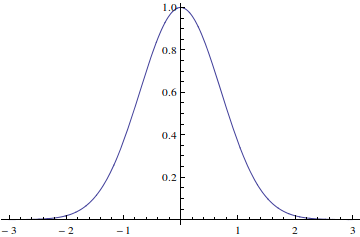
\includegraphics{img/bellcurve.png}
    \caption{Generated in Mathematica with following code:
      \texttt{Plot[E\^{}(-x\^{}2), \{x, -3, 3\}]}}
  \end{figure}
\end{enumerate}
